\documentclass[11pt]{amsart}
\usepackage{amssymb,amsmath,latexsym,times,enumitem,tikz,soul}

\setstcolor{red}
\setul{0pt}{1.5pt}

\addtolength{\evensidemargin}{-40pt}
\addtolength{\oddsidemargin}{-40pt}
\addtolength{\textwidth}{80pt}
\addtolength{\textheight}{80pt}
\addtolength{\topmargin}{-40pt}

\pagestyle{empty}

\begin{document}

\noindent
{\textbf{\color{blue}Charlene R. Ramos}}\\
ECON 280 Computation Fall 2024\\
Part \# 4: Extensions\\
Friday, December 6, 2024\\

\smallskip 

\noindent Bloom, Nicholas, Charles I. Jones, John Van Reenen, and Michael Webb. ``Are Ideas Getting Harder to Find?'' \emph{American Economic Review} 2020, 110 (4): 1104–1144.\\ 

\noindent {\textbf{\color{blue}Description of Extension}}

\smallskip

\noindent In Bloom et al. (2020), the authors use mean personal income from the Current Population Survey for males with a bachelor's degree or more of education to estimate the effective number of researchers. This variable is of particular interest for growth accounting purposes, since idea-based models examine economic growth as the byproduct of research productivity and number of researchers. The extension proposed here deflates gross domestic investment by a measure of the nominal wage considering high-skilled workers with a doctorate degree only. Although the majority of researchers presumably hold a bachelor's degree, many of them probably earned graduate degrees as well, which usually command higher wages in the labor market. Replacing such values from 1991 through 2014 results in a significant downward adjustment, with factor increase since 1930 becoming less steep, which suggests that Bloom et al. (2020) may be overestimating research effort by capturing less heterogeneity than available.

\bigskip

\noindent {\textbf{\color{blue}Original Figure 1}}

\smallskip

\begin{figure}[h]
    \centering 
    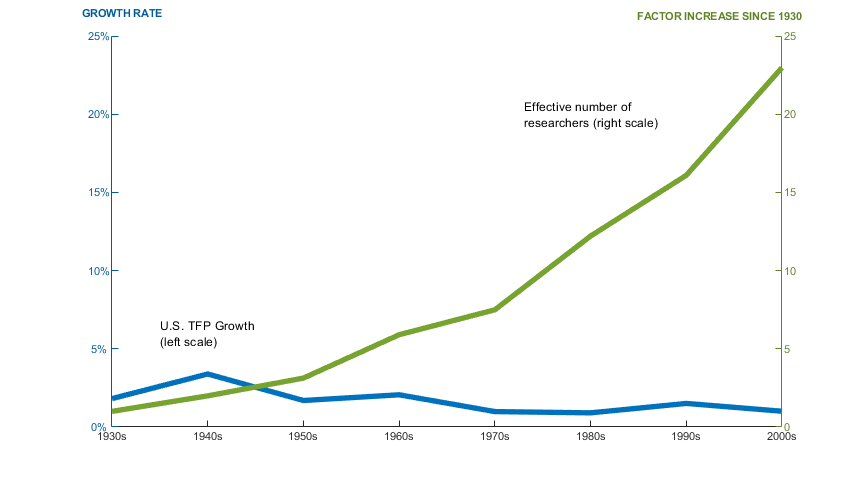
\includegraphics[width=0.64\textwidth]{factor.png}  
    \label{fig:histogram} 
\end{figure}

\noindent

\smallskip

\noindent {\textbf{\color{blue}Updated Figure 1 with Extension}}

\smallskip

\begin{figure}[h]
    \centering 
    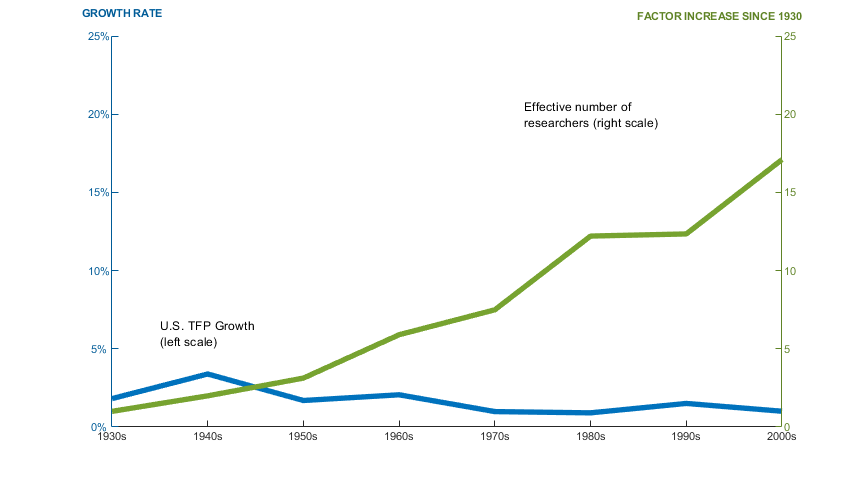
\includegraphics[width=0.64\textwidth]{factorCR.png}  
    \label{fig:histogram} 
\end{figure}

\end{document}

